% =====================================================================
%  第 6 章 §6.6 末段（Floer 同调与镜像对称）
%  ch06e2 —— 页段：PDF 373–382（原书 p.363–372）＋ 第 6 章章末评注
%  本块不是章首也不是节首：直接续写正文
% =====================================================================

% [原文 p.363]
\begin{figure}[htbp]
  \centering
  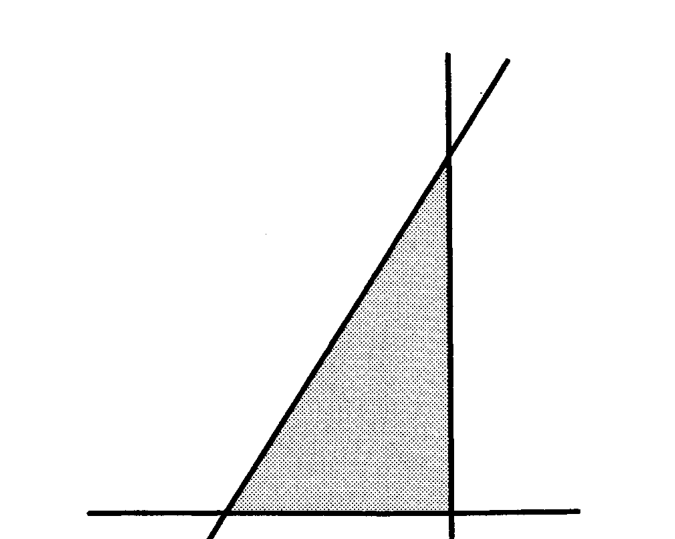
\includegraphics[width=0.34\textwidth]{figures/fig6.26.png}
  \figtitle{6.26}{伪全纯三角形（原书 p.363）}
\end{figure}

\begin{figure}[htbp]
  \centering
  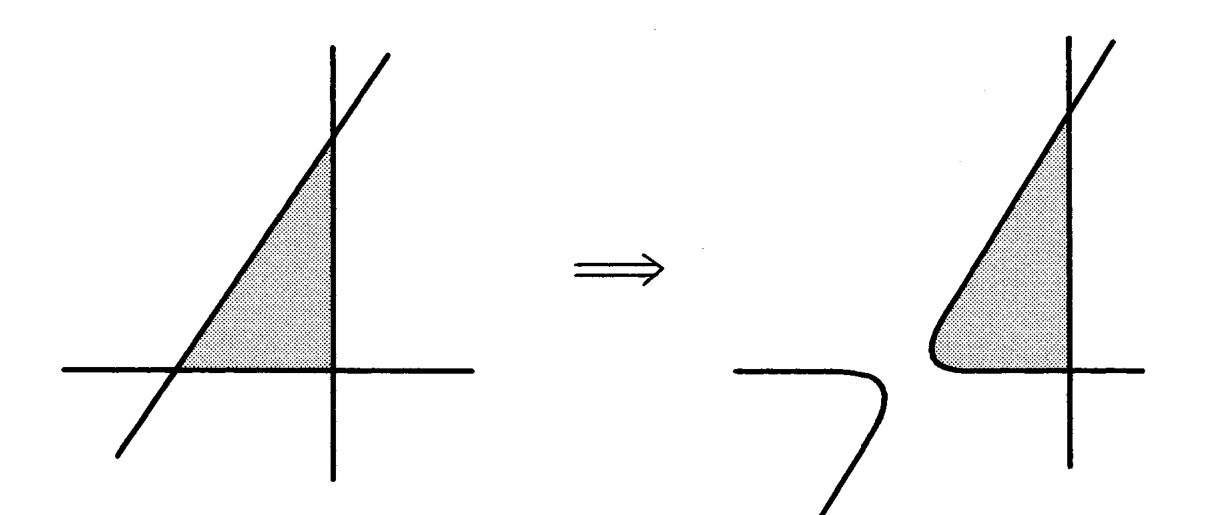
\includegraphics[width=0.62\textwidth]{figures/fig6.27.png}
  \figtitle{6.27}{拉格朗日手术与伪全纯圆盘（原书 p.363）}
\end{figure}

\begin{lemma*}{6.242}
  满足 (6.79) 的映射 $\varphi$ 的同伦类，与 $\pi_1(T^4)/\pi_1(L_{\mathrm{pt}}(v))\simeq\Z^2$ 一一对应。
\end{lemma*}

\begin{proof}
  在万有覆盖空间 $\C^2$ 中考虑。把 $L_{\mathrm{st}},L_{\mathrm{pol}}$ 提升为过 $0$ 的 $\tilde L_{\mathrm{st}},\tilde L_{\mathrm{pol}}$。对满足 (6.79) 的 $\varphi$，取其提升 $\tilde\varphi\colon\mathfrak{h}\to\C^2$ 使 $\tilde\varphi([-1,0])\subset\tilde L_{\mathrm{st}}$、$\tilde\varphi((-\infty,-1])\in\tilde L_{\mathrm{pol}}$。于是 $\tilde\varphi((0,\infty])$ 含于 $L_{\mathrm{pt}}(v)$ 的逆像的某个连通分支中。$L_{\mathrm{pt}}(v)$ 在 $\C^2$ 中的逆像，在 $\pi_1(T^4)/\pi_1(L_{\mathrm{pt}}(v))\simeq\Z^2$ 的元素的作用下彼此互换，故得引理。
\end{proof}

% [Tutor Note: 这里的计数是“指标”式的：$L_{\mathrm{pt}}(v)$ 是 $T^4$ 中的拉格朗日环面，$\pi_1(L_{\mathrm{pt}}(v))\subset\pi_1(T^4)$ 是秩 2 子格，商 $\Z^2$ 的每个元素恰好对应一族相差覆盖变换的圆盘，故同伦类与商群一一对应。]

\begin{lemma*}{6.243}
  满足 (6.79) 的伪全纯圆盘，在每个同调类中恰有一个。
\end{lemma*}

\begin{proof}
  忘掉辛结构、只考虑复结构，则 $T^4$ 与 $L_{\mathrm{pt}}(v),L_{\mathrm{st}},L_{\mathrm{pol}}$ 是图 6.24 的图形的直积。（辛结构与伪全纯映射模空间的定义无关。）以图 6.24 的图

  % [原文 p.364]
  形为边界值的伪全纯圆盘的条数显然是 $1$。由此即得引理。
\end{proof}

\begin{figure}[htbp]
  \centering
  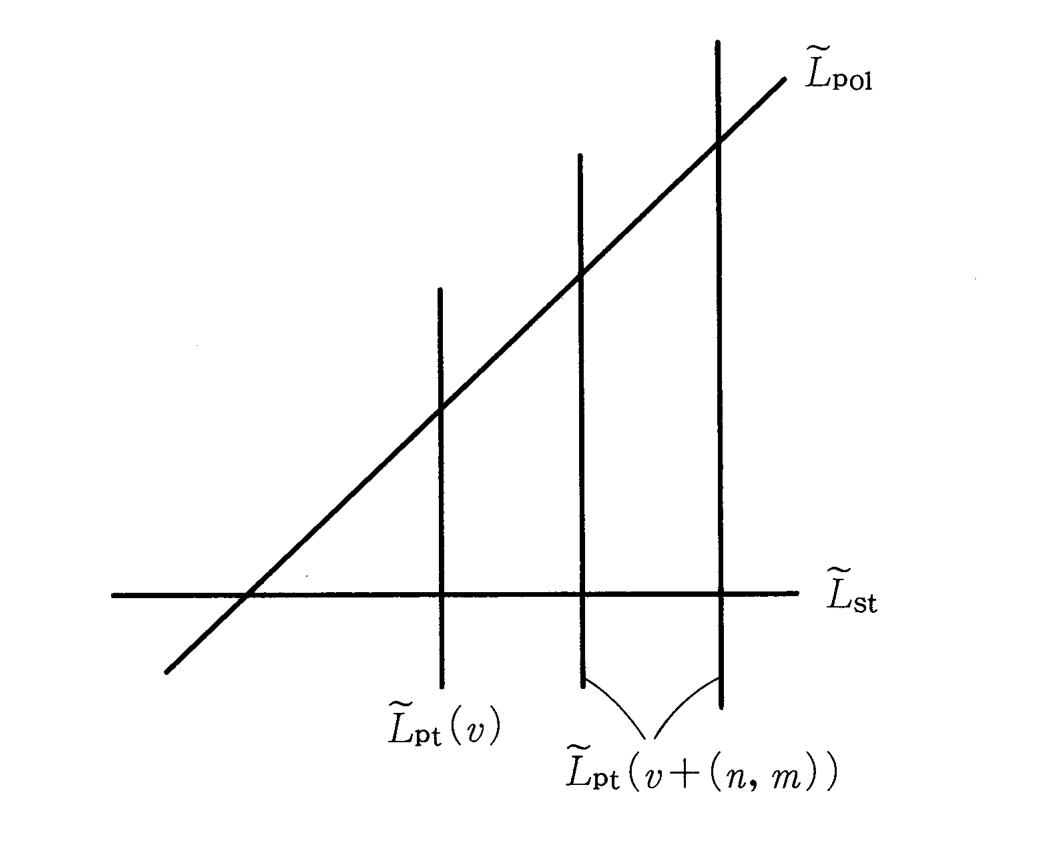
\includegraphics[width=0.52\textwidth]{figures/fig6.28.png}
  \figtitle{6.28}{由圆盘出发的映射的提升（原书 p.364）}
\end{figure}

这样，伪全纯圆盘的条数就清楚了。对每个同调类 $\in\Z^2$，权重随之确定。先设 $\alpha=0$。此时权重由伪全纯圆盘上 $\tilde\omega_{A,B}$ 的积分确定。这容易算出，累加起来便得下述函数。
\begin{equation}
  \vartheta(v,0)=\sum_{n,m}\exp\left(-\frac12\big\langle(v+(n,m)),(A+2\pi\sqrt{-1}B)(v+(n,m))\big\rangle\right) \tag{6.80}
\end{equation}
（$\langle\cdot,\cdot\rangle$ 指通常的欧氏内积。）

说明 $\alpha$ 存在时边界算子 $\delta$ 的定义。此时把 $\delta$ 看作映射 $\delta_{p,q}\colon\mathcal{L}_p^\alpha\to\mathcal{L}_q^\alpha$。（$\mathcal{L}^\alpha$ 是 $L_{\mathrm{pt}}(v)$ 上的平坦丛，其联络由 $\alpha$ 给出。$L$ 上考虑平凡联络。当考虑 $L$ 上具有非平凡联络的丛 $\mathcal{L}'$ 时，$\delta_{p,q}\colon\operatorname{Hom}(\mathcal{L}'_p,\mathcal{L}^\alpha_p)\to\operatorname{Hom}(\mathcal{L}'_q,\mathcal{L}^\alpha_q)$。）$\delta_{p,q}$ 定义如下。取伪全纯映射 $\varphi\colon\R\times[0,1]\to T^4$ 使
\begin{equation}
  \resizebox{0.97\linewidth}{!}{$\displaystyle \varphi(\R\times\{0\})\subset L_{\mathrm{pt}}(v),\qquad \varphi(\R\times\{1\})\subset L, \qquad \lim_{\tau\to-\infty}\varphi(\tau,t)=p,\qquad \lim_{\tau\to+\infty}\varphi(\tau,t)=q $} \tag{6.81}
\end{equation}

% [原文 p.365]
成立。（用 $\mathfrak{h}\simeq\R\times[0,1]$ 搬运，(6.78) 与 (6.81) 等价。）用 $Pal_\gamma^\alpha$ 表示关于联络 $\alpha$、沿道路 $\gamma$ 的平行移动，令
\[
  W(\varphi)=\exp\left(-\int_{\R\times[0,1]}\varphi^*\tilde\omega_{A,B}\right)
  Pal^\alpha_{\varphi|_{\R\times\{0\}}}
\]
（$W(\varphi)\colon\mathcal{L}_p^\alpha\to\mathcal{L}_q^\alpha$）。用 $W(\varphi)$ 定义 $\partial_{p,q}\colon\mathcal{L}_p^\alpha\to\mathcal{L}_q^\alpha$ 为
\begin{equation}
  \delta_{p,q}=\sum_{\varphi\ \text{为满足 (6.81) 的伪全纯映射}}W(\varphi) \tag{6.82}
\end{equation}
（不过求和取在由 $\R$ 方向的平移所定的 $\R$ 作用之下的、$\varphi$ 们的 $\R$ 等价类上。）

\begin{figure}[htbp]
  \centering
  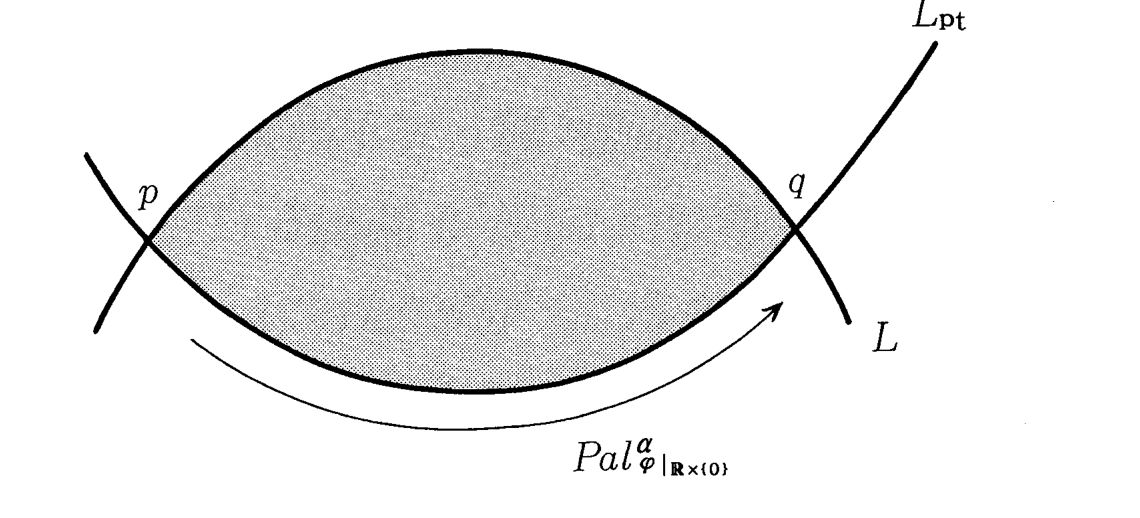
\includegraphics[width=0.58\textwidth]{figures/fig6.29.png}
  \figtitle{6.29}{带平坦丛时的边界算子（原书 p.365）}
\end{figure}

$\mathcal{L}^\alpha$ 为具平凡联络的平凡丛时，把 $Pal^\alpha_{\varphi|_{\R\times\{0\}}}$ 从 $W(\varphi)$ 的定义中删去后的 (6.82) 之和，就是 §5.4 的边界算子的定义，而在我们的情形化为 (6.80)。$\alpha$ 存在时，(6.82) 由下式表出。
\begin{equation}
  \resizebox{0.97\linewidth}{!}{$\displaystyle \vartheta(v,\alpha)=\sum_{n,m}\exp\left(-\frac12\big\langle v+(n,m),(A+2\pi\sqrt{-1}B)(v+(n,m))\big\rangle +2\pi\sqrt{-1}\big\langle(v+(n,m)),\alpha\big\rangle\right) $} \tag{6.83}
\end{equation}
(6.83) 就是 $\langle\delta[p],[q]\rangle$ 处的 theta 函数。

\begin{remark}{6.244}
  $\alpha$ 与 $\alpha+2\pi(n,m)$（$n,m\in\Z$）表示同一平坦联络。但要把这两者同一视之，需要规范变换。经规范变换，

  % [原文 p.366]
  $\operatorname{Hom}(\mathcal{L}_p,\mathcal{L}_q)$ 与 $\C$ 的同一视方式改变，因此 (6.83) 按 $\alpha\mapsto\alpha+2\pi\sqrt{-1}(n,m)$ 变化。这个变化式与 theta 函数的函数方程
  \[
    \vartheta(v,\alpha+(n,m))=\exp(2\pi\sqrt{-1}(v_1n+v_2m))\vartheta(v,\alpha)
  \]
  一致。（$\vartheta(v,\alpha)$ 关于 $v$ 是周期的。）
\end{remark}

\begin{remark}{6.245}
  发现 theta 函数与 Floer 同调、同调镜像对称之关系的是 Kontsevich [219]。[219] 中，对椭圆曲线情形证明了图式 (6.76) 第 2 行的映射是 theta 函数。

  Polishchuk–Zaslow [305]、Polishchuk [306] 更详细地考察了椭圆曲线的情形，证明了直到图式 (6.76) 的可交换性为止的椭圆曲线同调镜像对称。
\end{remark}

下面叙述定理 6.240 在同调镜像对称中的意义。(6.82) 的 $\vartheta(v,\alpha)$ 关于定义 6.235 的复结构是全纯的，给出 $(T^4,J_{AB})$ 上正（全纯）线丛 $\mathcal{L}_{\mathrm{pol}}$ 的截面。设 $\Sigma$ 为使 $\vartheta(v,\alpha)$ 为 $0$ 的 $(T^4,J_{AB})$ 的点全体之集合，即 theta 因子（theta divisor）。众所周知，$\Sigma$ 是亏格 $2$ 的黎曼面，而 $(T^4,J_{AB})$ 是它的 Jacobi 簇（Jacobi variety）。（引理 6.239 由此得出。）令 $\mathfrak{F}_\Sigma=i_*\mathcal{O}_\Sigma$。$i\colon\Sigma\to T^4$ 是嵌入，$\mathcal{O}_\Sigma$ 是 $\Sigma$ 的结构层。把 $(v,\alpha)$ 看作 $(T^4,J_{AB})$ 的点，对应的点层记作 $\mathfrak{F}_{p(v,\alpha)}$。由定理 6.240，下述同构成立：
\[
  \operatorname{Ext}\big(\mathfrak{F}_{p(v,\alpha)},\mathfrak{F}_\Sigma\big)
  \simeq HF\big((L_v,\mathcal{L}^\alpha),(L,\C)\big).
\]
按注 6.233 所述的想法，同调镜像对称下 $(L,\C)$ 的镜像是 $\mathfrak{F}_\Sigma$。即拉格朗日子流形 $L$ 在同调镜像对称下对应到 theta 因子的结构层。因此，例如下述同构应当成立。
\begin{equation}
  \operatorname{Ext}\big(\mathfrak{F}_\Sigma,\mathfrak{F}_\Sigma\big)
  \simeq HF\big((L,\C),(L,\C)\big). \tag{6.84}
\end{equation}
由于不存在以 $L$ 为边界的伪全纯圆盘，Floer 同调没有量子修正，因此 $HF((L,\C),(L,\C))$ 就是 $L$ 即亏格 $2$ 曲面的普通上同调。它与 $\operatorname{Ext}(\mathfrak{F}_\Sigma,\mathfrak{F}_\Sigma)$ 一致，这一点容易

% [原文 p.367]
验证\footnote{注 6.233 只是“想法”，(6.83) 的严格证明并不能由注 6.233 直接得到，需要另外验证。}。

% [Tutor Note: 这一段是同调镜像对称在 $T^4$ 上的具体兑现：B 模型一侧是 theta 因子（亏格 2 曲线）的结构层及其 Ext，A 模型一侧是 Floer 同调。要点是 $L$ 的边界上没有伪全纯圆盘，故 Floer 同调不含量子修正，两边退化为普通上同调而可直接比对。]

用同样的做法，可以构造模空间上确实发生量子形变（仓西映射不为 $0$）的例子，以及 Floer 同调的跨墙例子等，下面加以解说。

首先构造前者的例子。这回考虑 $T^6=\C^3/(\Z[\sqrt{-1}])^3$。取 $z_1=x_1+\sqrt{-1}y_1$、$z_2=x_2+\sqrt{-1}y_2$、$z_3=x_3+\sqrt{-1}y_3$ 为坐标。设 $A=(a^{ij})$、$B=(b^{ij})$ 为对称 $3\times3$ 矩阵，令 $\tilde\omega=\sum a^{ij}dx_i\wedge dy_j+2\pi\sqrt{-1}\sum b^{ij}dx_i\wedge dy_j$。$L_{\mathrm{pt}}(v)$ 由 $x_1=y_1$、$x_2=y_2$、$x_3=y_3$ 确定，$L_{\mathrm{st}}$ 由 $y_1=y_2=y_3=0$ 确定，$L_{\mathrm{pol}}$ 由 $x_1=y_1$、$x_2=y_2$、$x_3=y_3$ 确定。三个拉格朗日子流形中，任何两个都交于 $1$ 点。在 3 点处作拉格朗日手术所得的拉格朗日子流形记作 $L(v)$。因为是 $3$ 维的，拉格朗日手术的方式有 $2^3=8$ 种。选取 $L(v)$ 与由 $x_2=y_2$、$x_3=y_4$ 确定的 $T^2$ 的交集使之如图 6.30\footnote{$L(v)$ 可定向，但在复 $2$ 维情形对三个仿射拉格朗日子流形作同样的手术，会得到不可定向的拉格朗日子流形。}。把 $L(v)$ 在 $\C^3$ 中的逆像的连通分支记作 $\tilde L(v)$。$\pi_2(\C^3;\tilde L(v))\to H_2(\C^3;\tilde L(v))$ 的像是 $\Z^4$，由对应 3 处拉格朗日手术的消没圈 $\beta_1,\beta_2,\beta_3$ 以及图 6.31 的 $\beta$ 这 4 个生成。由于 $\int_{\beta_i}\tilde\omega_{A,B}=0$（$i=1,2,3$），权重由 $\beta$ 的系数决定。与命题 6.241、引理 6.243 同样地讨论，可对 $(L(v),\alpha)$ 求出 $m_0(1)$ 如下。

\begin{theorem}{6.246}
  \[
  \begin{aligned}
    m_0(1)=\sum_{\vec n\in\Z^3}\exp\Big(&-\frac12\big\langle v+\vec n,(A+2\pi\sqrt{-1}B)(v+\vec n)\big\rangle\\
    &+2\pi\sqrt{-1}\big\langle(v+\vec n),\alpha\big\rangle\Big)[\ell]
  \end{aligned}
  \]
  这里 $[\ell]$ 是由 $\partial\beta$ 确定的 $H_1(L(v);\Z)$ 的元素。
\end{theorem}

定理 6.246 中没有动 $L_{\mathrm{st}},L_{\mathrm{pol}}$，但要得到 $\mathcal{LAG}_{\mathrm{st}}(T^6,\tilde\omega_{A,B})$ 的连通分支，须把它们也沿平行移动动起来。于是得到 $T^6\times T^6\times T^6$ 这样的

% [原文 p.368]
\begin{figure}[htbp]
  \centering
  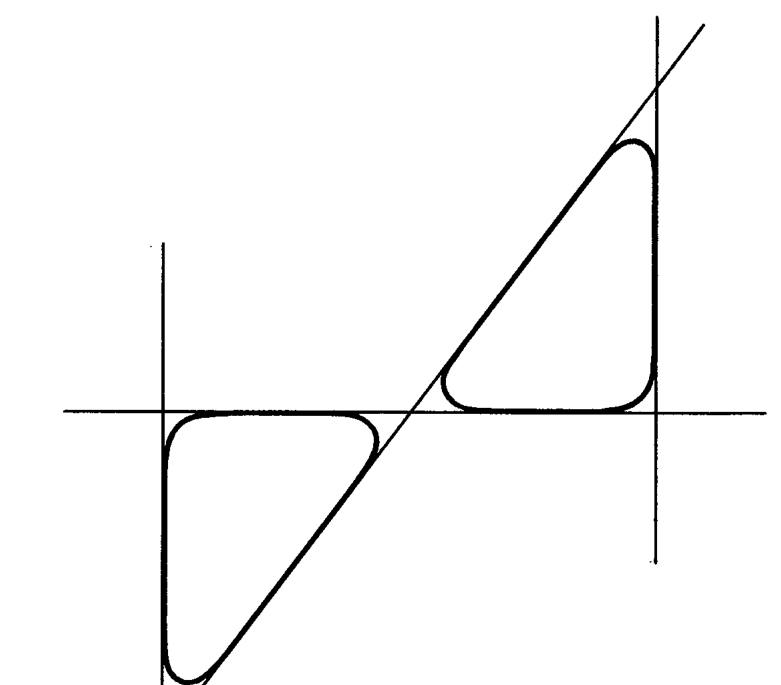
\includegraphics[width=0.42\textwidth]{figures/fig6.30.png}
  \figtitle{6.30}{$L(v)$ 的取法（原书 p.368）}
\end{figure}

\begin{figure}[htbp]
  \centering
  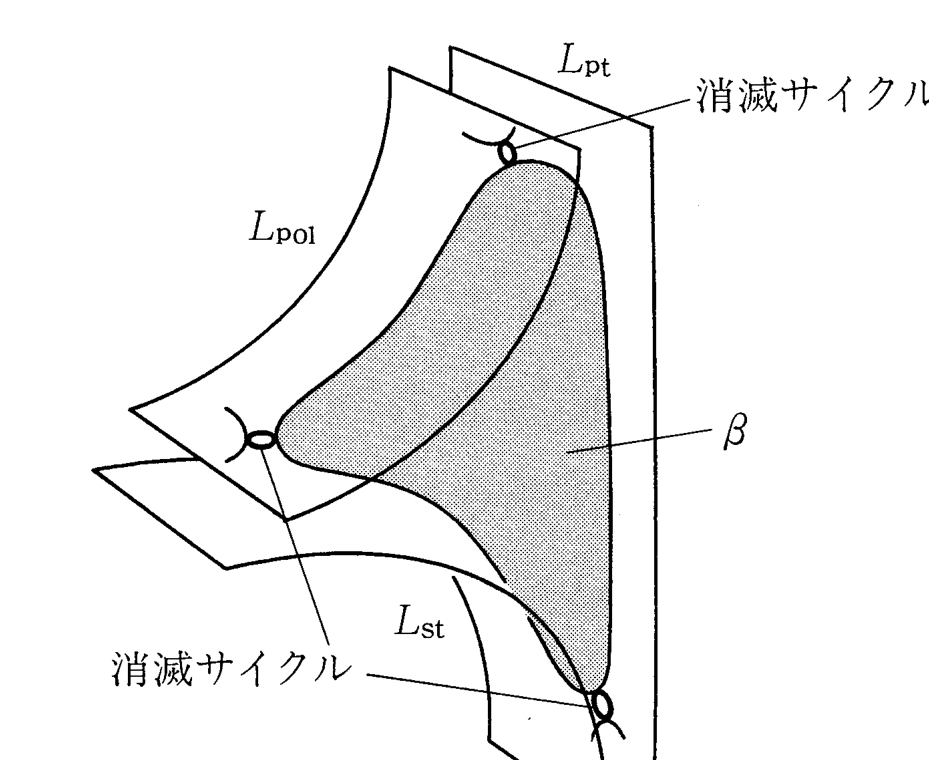
\includegraphics[width=0.48\textwidth]{figures/fig6.31.png}
  \figtitle{6.31}{$\pi_2(\C^3,\tilde L(v))$（原书 p.368）}
\end{figure}

$\mathcal{LAG}_{\mathrm{st}}(T^6,\tilde\omega_{A,B})$ 的连通分支。（3 个成分分别是与 $L_{\mathrm{st}},L_{\mathrm{pol}},L_{\mathrm{pt}}$ 平行的拉格朗日子流形的模空间。复结构是直积，在各成分上可与引理 6.234 同样地计算。）

对由 $((v^1,\alpha^1),(v^2,\alpha^2),(v^3,\alpha^3))\in T^6\times T^6\times T^6$ 变动所得的拉格朗日子流形族考虑 $m_0(1)$，它仍是 theta 函数，把它限制到 $(v^1,\alpha^1)=(v^2,\alpha^2)=0$ 所得的就是定理 6.246 的右边。（以下记作 $\vartheta_{A,B}(v,\alpha)$。）因此，$\mathcal{LAG}_{\mathrm{qm}}(T^6,\tilde\omega_{A,B})\subset\mathcal{LAG}_{\mathrm{st}}(T^6,\tilde\omega_{A,B})$ 与 $\{(\vec0,\vec0)\}\times T^6$ 的交集，就是 theta 因子 $\vartheta^{-1}_{A,B}(0)$。

% [Tutor Note: “量子形变”在这里的含义是：$\mathcal{LAG}_{\mathrm{qm}}$ 是 $\mathcal{LAG}_{\mathrm{st}}$ 中被 Floer 同调（即量子修正）真正改变的那部分，而它与某个切面的交不再是光滑点集，而是 theta 因子 $\vartheta^{-1}_{A,B}(0)$——这正是仓西映射不为 $0$ 的可见后果。]

% [原文 p.369]
它就是 $\vartheta^{-1}_{A,B}(0)$ 的镜像，即 $(T^6,J_{AB})$ 的凝聚层。$L_{\mathrm{st}},L_{\mathrm{pol}},(L_{\mathrm{pt}}(v),\alpha)$ 对应的层依次是结构层 $\mathcal{O}$、极化 $P$、点层 $\mathfrak{F}_{p(v,\alpha)}$。稍作说明：$P$ 是使 $\tilde\omega_{A,B}$ 成为其截面的正线丛，$p(v,\alpha)$ 是由 $(v,\alpha)$ 确定的镜像之点。考虑下列层之间的同态列。
\begin{equation}
  0\to\mathcal{O}\to P\to\mathfrak{F}_{p(v,\alpha)}\to0 \tag{6.85}
\end{equation}
这里 $\mathcal{O}\to P$ 由 $\tilde\omega_{A,B}$ 给出，$P\to\mathfrak{F}_{p(v,\alpha)}$ 由确定 $P$ 在 $p(v,\alpha)$ 处的纤维与 $\C$ 的同构而定。

(6.85) 定出层的复形，是在 $p(v,\alpha)$ 位于 theta 因子 $\vartheta^{-1}_{A,B}(0)$ 上之时。换言之，theta 因子 $\vartheta^{-1}_{A,B}(0)$ 构成层之复形的模空间。（把 $\mathcal{O},P$ 也在 $T^6$ 的对偶阿贝尔簇上变动，其全体就成为 $\mathcal{LAG}_{\mathrm{qm}}(T^6,\tilde\omega_{A,B})$ 的连通分支。）对应于 $p(v,\alpha)\in\vartheta^{-1}_{A,B}(0)$ 的凝聚层，由取 (6.85) 的上同调层得到。即：

\begin{proposition}{6.247}
  $(L_{\mathrm{pt}}(v),\alpha)$ 的镜像是 $i_*\mathcal{J}_{p(v,\alpha)}$。这里 $i\colon\vartheta^{-1}_{A,B}(0)\to T^6$ 是嵌入，$\mathcal{J}_{p(v,\alpha)}$ 是 $p(v,\alpha)\in\vartheta^{-1}_{A,B}(0)$ 的理想层\footnote{不是点层。}。
\end{proposition}

命题中的 $i_*\mathcal{J}_{p(v,\alpha)}$ 看上去应该像是 3-膜（实 $4$ 维复子流形）与 $(-1)$-膜（$0$ 维子流形）组合配置而成的东西。

命题 6.247 中出现的层本身并不有趣，但作为展现本节构造诸多侧面的具体例子却很有意思。在命题 6.247 的对应下，也可以确认 Floer 上同调与层系数上同调相对应（猜想 6.230）。此时 Floer 上同调 $HF(L(v,\alpha),L(v,\alpha))$ 并不等于 $H(L(v);\C)$。

最后举出 Floer 同调跨墙的例子。伪全纯圆盘模空间跨墙的最易看出的例子，当属 Polishchuk 在 [306] 中指出的下例。考虑 $\C$ 上实的 $1$ 维子流形 $L_1,\dots,L_4$，把 $L_3$ 与 $L_4$ 分别只平移 $v\in\R\simeq\C/L_3$、$w\in\R\simeq\C/L_4$ 后的东西记作 $L_3(v),L_4(w)$（图 6.32）。考虑满足下述条件的 $\varphi\colon D^2\to\C$ 与 $(z_1,\dots,z_4)\in\partial D^2$ 之组全体 $\mathcal{M}_{0,4}(\C;L_1,L_2,L_3(v),L_4(w))$。

% [原文 p.370]
\begin{figure}[htbp]
  \centering
  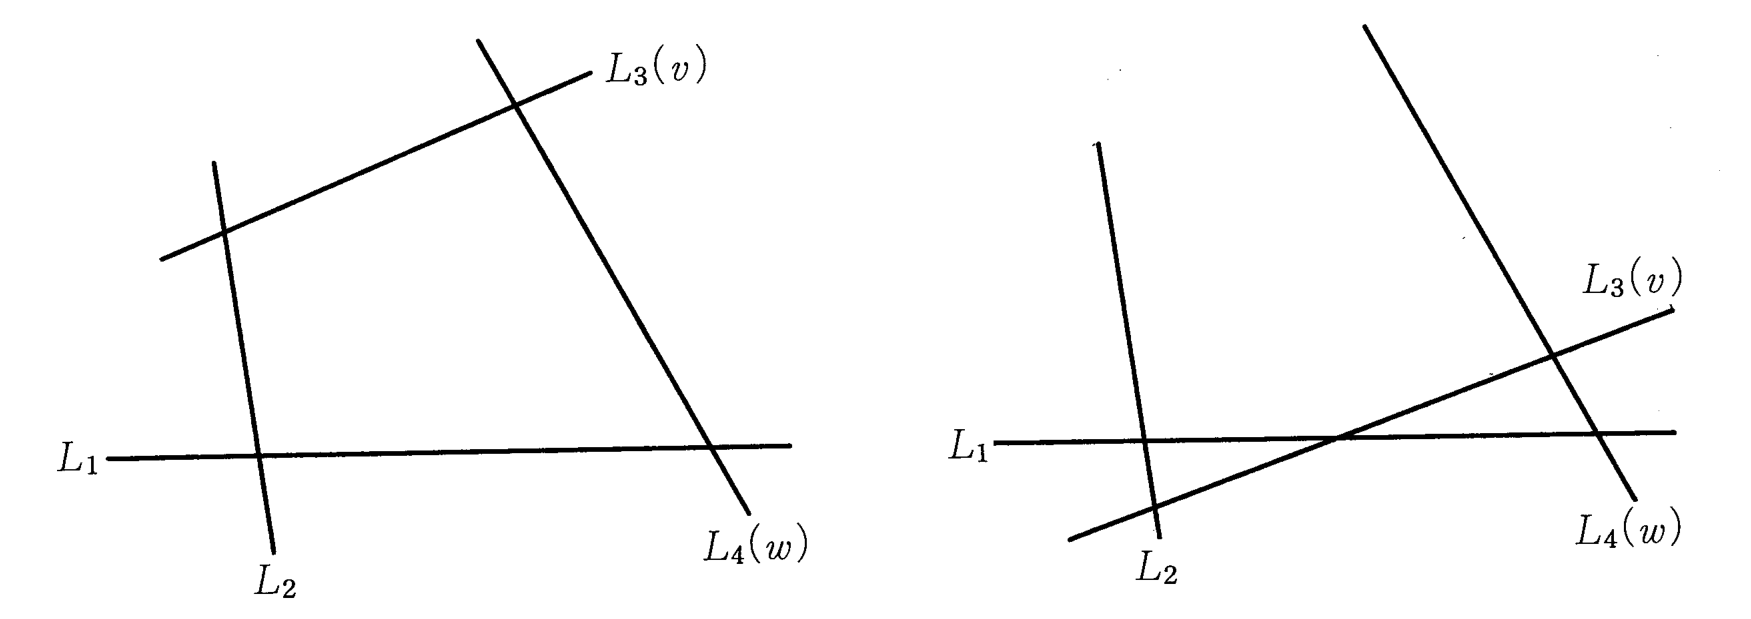
\includegraphics[width=0.74\textwidth]{figures/fig6.32.png}
  \figtitle{6.32}{四片仿射拉格朗日子流形（原书 p.370）}
\end{figure}

\begin{assumption}{6.248}
  \begin{enumerate}[label=（\arabic*）,leftmargin=2.4em]
    \item $\varphi$ 是伪全纯的。
    \item $\varphi(z_i)\in L_i\cap L_{i+1}$。（但视 $L_5=L_1$。）
    \item $z_1,\dots,z_4$ 在圆周 $\partial D^2$ 上按时针方向排列。
    \item 设 $\widehat{z_iz_{i+1}}$ 为 $\partial D^2$ 上 $z_i$ 与 $z_{i+1}$ 之间的部分，则 $\varphi(\widehat{z_iz_{i+1}})\in L_i$。
  \end{enumerate}
\end{assumption}

由图 6.33 容易看出，$\mathcal{M}_{0,4}(\C;L_1,L_2,L_3(v),L_4(w))$ 是空集或只有 $1$ 点；使 $\mathcal{M}_{0,4}(\C;L_1,L_2,L_3(v),L_4(w))$ 非空的 $(v,w)$ 的集合成图 6.33 那样的图形\footnote{由 Riemann 映射定理显然。}。值得注意的是，在图 6.33 的边界点处，集合 $\mathcal{M}_{0,4}(\C;L_1,L_2,L_3(v),L_4(w))$ 的个数会不连续地变化。

\begin{figure}[htbp]
  \centering
  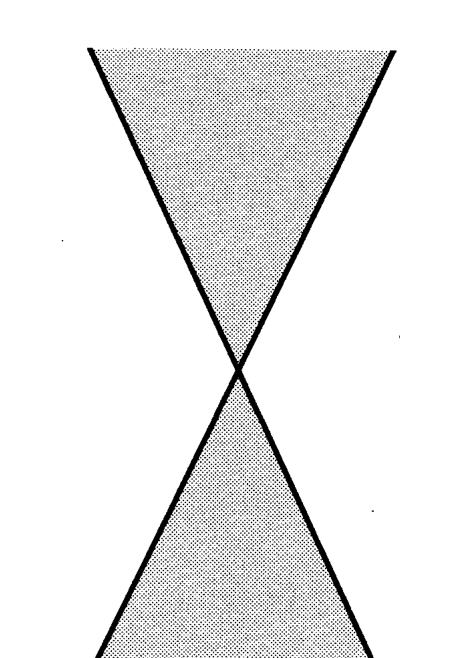
\includegraphics[width=0.30\textwidth]{figures/fig6.33.png}
  \figtitle{6.33}{$\mathcal{M}_{0,4}(\C;L_1,L_2,L_3(v),L_4(w))$ 何时为空（原书 p.370）}
\end{figure}

% [Tutor Note: 条件 6.248 的 (3) 是“按时针方向”，(4) 规定相邻两点之间的弧映到同一条 $L_i$。这两条合起来把圆盘的边界按 $L_1,L_2,L_3,L_4$ 的顺序依次贴住，故拓扑上只能给出单调四边形；一旦 $(v,w)$ 越过某条边界线，可贴的圆盘便整体消失——这就是“跨墙”的最简模型。]

% [原文 p.371]
这个例子可以高维化。即把 4 片仿射拉格朗日子流形在 $\C^n$ 上变动，同样地定义 $\mathcal{M}_{0,4}(\C^n;L_1,L_2,L_3(v),L_4(w))$。考虑固定 $v,w\in\R^n$ 时模空间 $\mathcal{M}_{0,4}(\C^n;L_1,L_2,L_3(v),L_4(w))$ 的虚拟维数为 $0$ 的情形。

固定 $v,w\in\R^n$，则 $\mathcal{M}_{0,4}(\C^n;L_1,L_2,L_3(v),L_4(w))$ 是 $1$ 点或空。而且，使 $\mathcal{M}_{0,4}(\C^n;L_1,L_2,L_3(v),L_4(w))$ 非空的 $(v,w)\in\R^{2n}$ 的全体，成为由 2 张超平面围成的、与图 6.33 同样的图形。

\begin{remark}{6.249}
  这一结论的证明与 $1$ 维情形不同，并不初等。（仅靠 Riemann 映射定理不能给出。）证明可由 [121] 与 [122] 合起来得到。要点是归约到二次函数的 Morse 理论 [123]。
\end{remark}

对 4 片以上的仿射拉格朗日子流形，类似的结果也成立。仿射拉格朗日子流形增多时，相当于图 6.33 的区域中会出现各种各样的东西。

考虑 $\C^2$ 的 4 张拉格朗日平面，把它们看作 $T^4$ 的拉格朗日环面。两张两张地用拉格朗日手术连接起来，便得到两个亏格 $2$ 曲面的拉格朗日子流形。其间的 Floer 同调的边界算子，与 3 张的情形同样，可通过考察 $\mathcal{M}_{0,4}(\C^n;L_1,L_2,L_3(v),L_4(w))$ 来计算。答案是：把图 6.33 的 $4$ 维版的阴影部分区域记作 $D$，
\begin{equation}
  \sum_{(v,w)+\vec n\in D}
  \exp\left(-\frac12\big\langle((v,w)+\vec n),(Q+2\pi\sqrt{-1}R)((v,w)+\vec n)\big\rangle\right) \tag{6.86}
\end{equation}
其中 $Q$ 是正特征值个数为 $3$、负特征值个数为 $1$ 的二次形式，且在 $(v,w)+D$ 上取正值。

(6.86) 是不定二次形式的 theta 函数。正如 Polishchuk 在 [306] 中所注意到的，$1$ 维情形 (6.86) 的类似物的特殊情形（$L_1$ 与 $L_3$、$L_2$ 与 $L_4$ 平行的情形）会得到 Kronecker 的二重 theta 级数（double theta series，见 [383]）。推广到高维，便得到几乎处处不连续的 theta 函数的推广（多重 theta 函数（multi theta function））。它们描述阿贝尔簇上向量丛上同调的高阶 Massey

% [原文 p.372]
积。以上所述之事，就是拉格朗日环面中、仿射拉格朗日流形及其拉格朗日手术情形的同调镜像对称猜想，已在 [121] 中证明。

\chapterreview{%
第 6 章是全书的终点，也是唯一一章以“不变量”与“镜像对称”为主角的一章。前五章积累的工具——近复结构、伪全纯曲线、模空间与紧化、Floer 同调、拉格朗日配边——在此汇成两件成果：Gromov–Witten 不变量的严格定义，以及它在镜像对称中的计算价值。就全书的论证结构而言，前五章是准备，本章才是目的。

脉络可分三段。§6.1–§6.3 从物理图像出发，把 $A$ 模型的 Gromov–Witten 势写成形式幂级数，用 WDVV 方程族化出 Frobenius 流形，并以势函数在巨大体积极限附近的收敛性说明模空间如何被“量子形变”。§6.4–§6.5 转向 $B$ 模型，用同伦代数与形变理论把复结构的形变写成 $A_\infty$／$L_\infty$ 代数上的 Maurer–Cartan 方程，再经形变量子化与 operad 与之对接。§6.6 给出同调镜像对称的精确陈述，并在椭圆曲线、$T^4$、$T^6$ 等例上逐条验证，最后用 Polishchuk 的四条仿射直线说明跨墙。

核心结论有三。其一，Gromov–Witten 不变量是伪全纯曲线模空间的虚拟基本类上的积分，其存在性依赖第 2 章的紧化与第 3–5 章的 Kuranishi 型扰动。其二，WDVV 方程等价于 Frobenius 代数积的结合律，从而把无穷多计数关系压缩为一个方程；反过来，这个方程又足以推出 $\C P^2$ 的全部计数 $N(k)$。其三，同调镜像对称把 $A$ 侧的 Floer 同调与 $B$ 侧的凝聚层 Ext 群对应起来，在 $T^4$ 上表现为 theta 函数与 theta 因子的对偶，在 $T^6$ 上则表现为仓西映射不为零所带来的量子形变。

需要提醒的有两处。其一，本章大量使用“虚拟基本类”“Kuranishi 结构”这类技术，书中只给轮廓，真正的构造要到 [FOOO]；读时不要把 §6.6 的定理当成已完全证明的陈述。其二，镜像对称在成书之时（1999 年）仍是猜想，本章的“定理”多为在特例上的验证；2008 年的追记已修正若干处，读者应两处对读，尤其要注意引理 6.225 的循环对称性在 [FOOO] 的框架下反而不再成立这一点。

作者写法上，本章以物理直觉开路、以代数结构收束，气势最盛而技术细节最薄。这一取舍使全书有了统一的图景，代价是许多关键步骤只能诉诸文献：Kuranishi 结构、虚拟基本类、$A_\infty$ 算子的收敛性，书中都只给了名字与用途。就整本书而言，第 6 章不是终点而是入口：它把辛几何与代数几何、可积系统、量子场论接在一起，也正是作者在追记中所说“1999 年以后有诸多进展”而未能纳入的部分。读者若想继续，宜以本章所列文献为路标，再辅以 [FOOO] 与 Kontsevich 一系的原始论文。%
}

% CHUNK ch06e2 DONE
